
\documentclass{article} % For LaTeX2e
\usepackage[T1]{fontenc}
\usepackage{iclr2027_conference,times}

% Optional math commands from https://github.com/goodfeli/dlbook_notation.
\input{math_commands.tex}

\usepackage{hyperref}
\usepackage{url}
\usepackage{graphicx}
\usepackage{booktabs}
\usepackage{placeins}
\usepackage{wrapfig}

\title{MASOpt: Online Prompt Optimization for Multi-Agent Systems 
with Closed-Loop Control Theory}


% Authors must not appear in the submitted version. They should be hidden
% as long as the \iclrfinalcopy macro remains commented out below.
% Non-anonymous submissions will be rejected without review.

\author{Anonymous Authors}

% The \author macro works with any number of authors. There are two commands
% used to separate the names and addresses of multiple authors: \And and \AND.
%
% Using \And between authors leaves it to \LaTeX{} to determine where to break
% the lines. Using \AND forces a linebreak at that point. So, if \LaTeX{}
% puts 3 of 4 authors names on the first line, and the last on the second
% line, try using \AND instead of \And before the third author name.

\newcommand{\fix}{\marginpar{FIX}}
\newcommand{\new}{\marginpar{NEW}}

%\iclrfinalcopy % Uncomment for camera-ready version, but NOT for submission.
\begin{document}


\maketitle

\begin{abstract}
Large language model (LLM)-based multi-agent systems (MAS) have emerged as a powerful paradigm for complex problem solving, where prompts play a central role in shaping both individual agent behaviors and inter-agent coordination.
Existing MAS prompt optimization methods primarily optimize prompts before deployment and keep them fixed during execution, making them unable to adapt to errors and state changes revealed by an ongoing trajectory.
We introduce \textbf{MASOpt}, a framework for \textbf{online prompt optimization in multi-agent systems} inspired by classical closed-loop control theory.
MASOpt treats each prompt modification as a control action whose effectiveness must be determined from the subsequent system response.
A lightweight meta-MAS continuously diagnoses the current execution state, proposes local prompt repairs, and verifies their actual effects, allowing ineffective updates to be reverted and unresolved problems to trigger further optimization within the same episode.
To reduce online exploration, we further introduce \textbf{Cross-Actuation Relative Advantage (CARA)}, which compares alternative prompt interventions from matched execution states and learns state-conditioned repair preferences from historical trajectories without updating the underlying LLM parameters.
We formulate an evaluation protocol spanning question answering, code generation, mathematical reasoning, and interactive decision-making benchmarks. The protocol is designed to test whether online closed-loop repair improves over strong offline prompt-optimization baselines.

\end{abstract}

\section{Introduction}
\label{sec:introduction}

Large language model (LLM)-based multi-agent systems (MAS) have become a promising paradigm for solving complex tasks.
By assigning planning, reasoning, execution, and verification to specialized agents, MAS decompose difficult problems into coordinated sub-processes and combine the complementary capabilities of multiple LLM calls
\citep{wu2023autogen,li2023camel,chen2023agentverse,yao2024multiagent}.
Their effectiveness, however, depends not only on the underlying language models and workflow topology, but also on the prompts that govern individual agents.
Prompts determine how an agent interprets its role, consumes upstream information, and communicates with downstream agents.
Consequently, optimizing prompts has become a key mechanism for improving the performance of a fixed multi-agent system.

Prompt optimization in MAS is substantially more challenging than in a single-agent setting.
Different agents solve different sub-problems and therefore require role-specific instructions, while their behaviors remain strongly coupled through inter-agent communication.
A change to an upstream prompt can alter the input distribution seen by several downstream agents, making an individually improved prompt potentially harmful to the overall workflow.
Moreover, the appropriate instruction for an agent may depend on the execution state reached by a particular task.
An instruction that is useful early in a trajectory may become irrelevant or even counterproductive after new evidence, tool outputs, or execution failures emerge.
This suggests a more desirable form of prompt optimization in which prompts are not treated as immutable parameters of an episode, but can adapt to the evolving state of the task.

Existing MAS prompt optimization approaches can be broadly grouped into two paradigms.
The first optimizes prompts for individual agents using local feedback or generic prompt optimizers.
Such methods are simple and effective, but they largely ignore dependencies among agents.
The second performs system-level optimization and explicitly considers interactions across the workflow.
Recent approaches such as MAPRO, MASPOB, and MASPO model topology-aware feedback, joint prompt quality, or downstream utility to obtain better coordinated prompt configurations
\citep{mapro2026,hong2026maspob,wang2026maspo}.
Despite their different optimization strategies, both paradigms share the same basic assumption.
Prompt optimization is performed before deployment, after which the resulting prompts are used as a largely fixed configuration for a complete execution.
The partial trajectory of a new task therefore has limited ability to change the prompts that govern the remainder of that task.
As MAS are increasingly used for long-horizon and dynamic problems, moving prompt optimization from a purely offline procedure to an online process becomes a natural next step.

\begin{figure}[t]
    \centering
    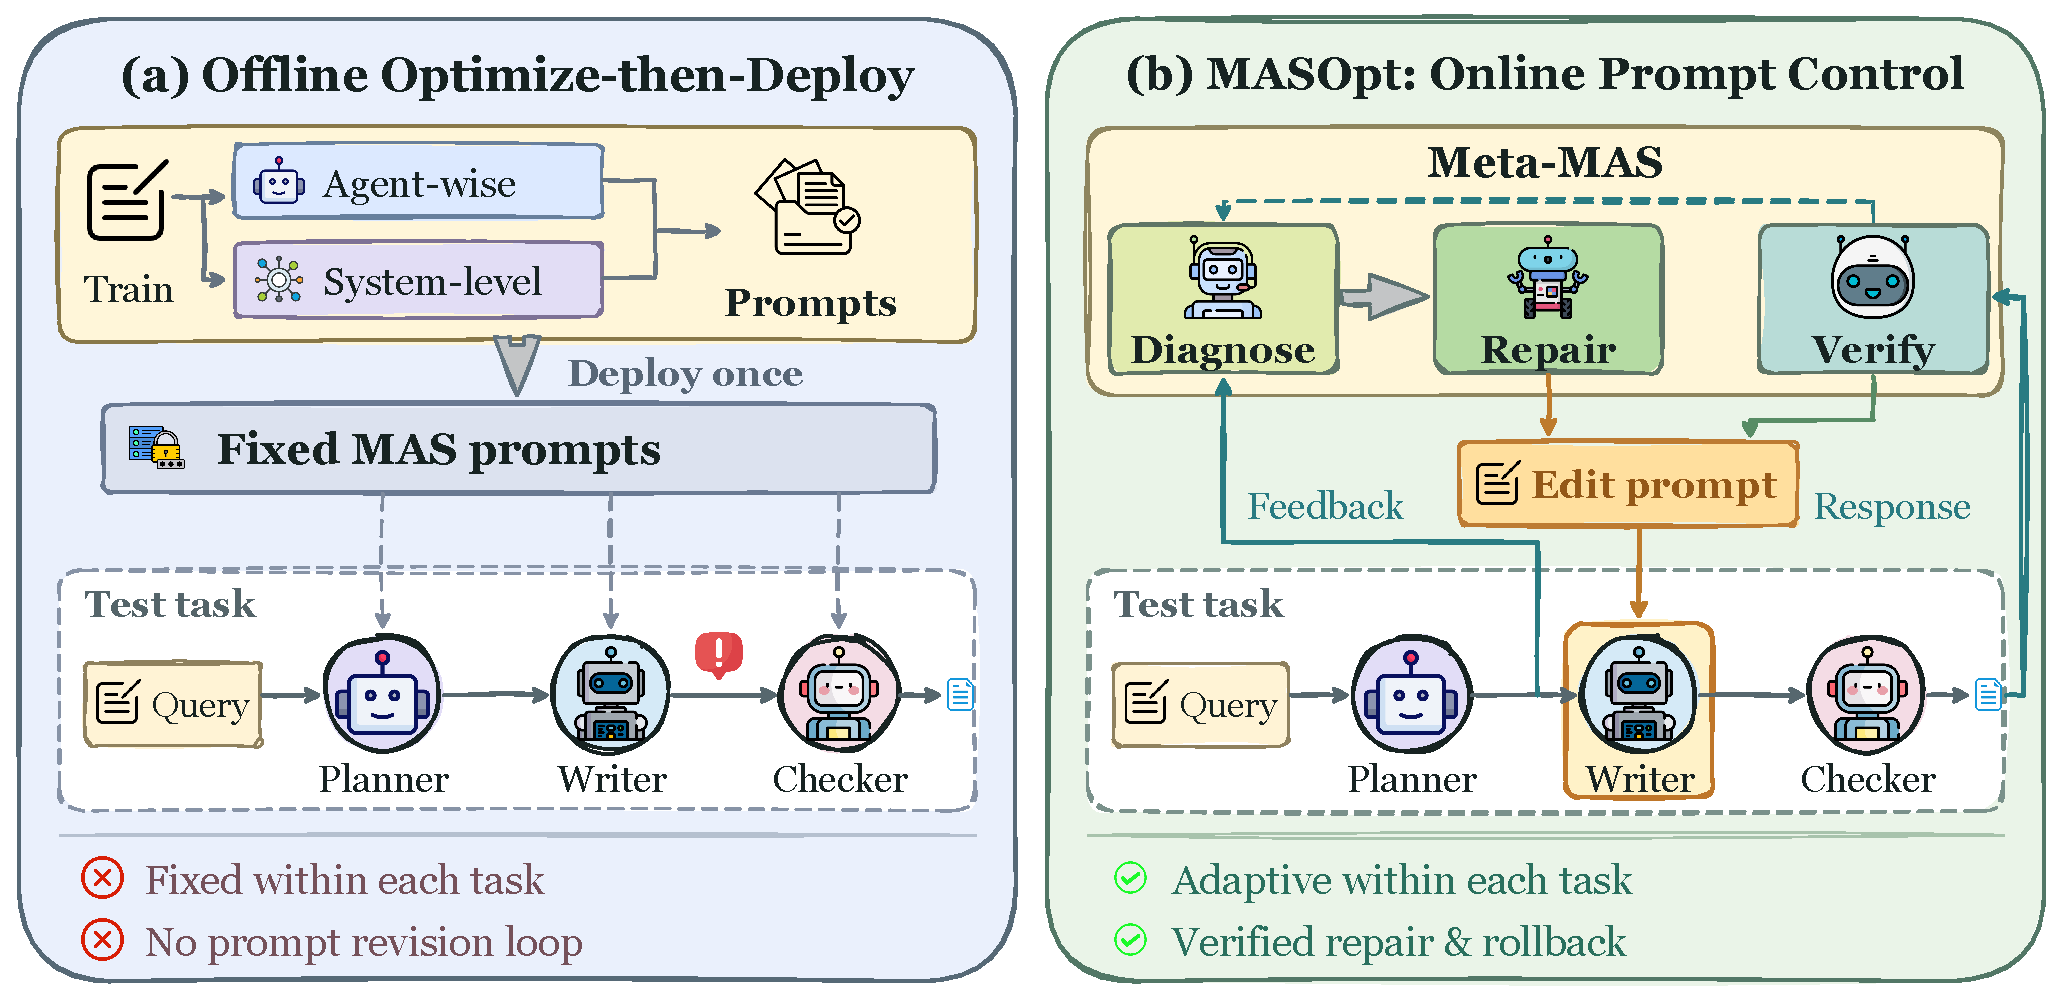
\includegraphics[width=\linewidth]{figures/masopt_introduction_comparison.pdf}
    \caption{Offline prompt optimization and online closed-loop prompt control. \textbf{Left:} agent-wise and system-level optimizers produce a prompt configuration before deployment; that configuration remains largely fixed during a new task. \textbf{Right:} MASOpt uses a Diagnose--Repair--Verify meta-MAS to adapt prompts within the current task. Runtime feedback motivates a local intervention, and its observed effects determine whether to retain or roll back the change; residual feedback drives another round. The task and agent roles are illustrative.}
    \label{fig:masopt-paradigms}
\end{figure}

Online prompt optimization introduces a different challenge.
An intermediate trajectory may reveal that the system has deviated from a desirable behavior, but it does not directly specify how its prompts should be changed.
More importantly, a plausible prompt modification is not necessarily a correct one.
It may resolve the current error, have little effect, or introduce a new downstream failure.
This observation motivates us to view online prompt optimization through the lens of \textbf{closed-loop control theory}
\citep{astrom2008feedback,goodwin2001control}.
A closed-loop controller does not assume that a control action is correct in advance.
It applies an action, observes the resulting system response, and uses the new feedback to determine the next action.
We adopt the same principle for MAS prompt optimization.
Each prompt modification is regarded as a temporary control action.
Its value is determined only after observing how the target MAS responds to the modification.
Successful changes can be retained, harmful ones can be reverted, and partially resolved failures can generate new feedback for another optimization round.

Based on this view, we propose \textbf{MASOpt}, an online prompt optimization framework for multi-agent systems.
MASOpt places a lightweight meta-MAS around a running target MAS.
A \textbf{Diagnose Agent} interprets partial execution trajectories and converts observable failures into structured feedback.
A \textbf{Repair Agent} uses this feedback to construct a minimal local prompt intervention.
A \textbf{Verify Agent} evaluates the post-intervention behavior and determines whether the modification should be retained, reverted, or further refined.
To make this online process efficient, we additionally introduce \textbf{Cross-Actuation Relative Advantage (CARA)}.
During offline calibration, CARA compares alternative prompt interventions from the same execution checkpoint and estimates which types of repairs are more effective under different failure states.
The resulting experience is stored as reusable feedback-control memory and serves as a prior during online optimization.
The target LLMs and MAS topology remain unchanged throughout this process.
MASOpt therefore combines offline repair experience with online closed-loop feedback without requiring model-parameter updates.
Figure~\ref{fig:masopt-paradigms} contrasts this within-task adaptation with offline optimize-then-deploy prompting.

Our contributions are summarized as follows.
\begin{itemize}
    \item \textbf{Online MAS prompt optimization.}
    We introduce, to our knowledge, the first systematic formulation of online prompt optimization for multi-agent systems.
    Unlike conventional optimize-then-deploy approaches, MASOpt allows intermediate execution feedback from the current task to directly modify the prompts used by the remainder of the same task.

    \item \textbf{Closed-loop prompt control with CARA.}
    We formulate online MAS prompt optimization from the perspective of closed-loop control theory and develop a three-agent meta-MAS for diagnosis, repair, and verification.
    We further introduce Cross-Actuation Relative Advantage to learn state-conditioned repair preferences from matched execution states without updating the underlying LLM parameters.

    \item \textbf{Evaluation framework.}
    We specify an evaluation protocol spanning question answering, code generation, mathematical reasoning, and interactive decision-making tasks.
    The protocol isolates the contributions of online verification, matched-state probing, and CARA while avoiding unsupported performance claims before the benchmark runs are complete.
\end{itemize}

\section{Related Work}
\label{sec:related_work}

\subsection{Automatic Prompt and Program Optimization}

The strong sensitivity of LLMs to natural-language instructions has motivated a broad line of work on automated prompt optimization.
Early approaches such as Automatic Prompt Engineer generate and select instruction candidates using task-level evaluation
\citep{zhou2022ape,pryzant2023automatic}.
OPRO casts optimization itself as a language modeling problem, where an LLM proposes new solutions conditioned on previously evaluated candidates
\citep{yang2024opro}.
PromptBreeder adopts an evolutionary perspective and jointly evolves task prompts and the mutation prompts used to modify them
\citep{fernando2024promptbreeder}.
Other approaches optimize more structured language-model programs.
DSPy treats prompts and demonstrations as parameters of declarative LM pipelines and compiles them against task metrics
\citep{khattab2024dspy},
while TextGrad propagates textual feedback through compound AI systems in a manner analogous to automatic differentiation
\citep{yuksekgonul2024textgrad,agrawal2025textgrad}.
More recently, SkillOpt treats external agent skills as optimizable textual parameters while keeping the target model frozen
\citep{yang2026skillopt}.

These approaches establish that natural-language instructions can be optimized systematically without relying exclusively on manual prompt engineering. They also expose a recurring limitation: most optimization signals are collected at the level of complete trials, so the optimizer receives little information about when a prompt becomes harmful within a trajectory.
However, most of them optimize prompts or textual parameters using an offline development process and subsequently deploy the selected configuration.
MASOpt instead focuses on prompt adaptation \emph{during} the execution of a new multi-agent task.


\subsection{System-Level Prompt Optimization for Multi-Agent Systems}

Prompt optimization becomes more difficult in MAS because prompts interact through the workflow topology.
Optimizing one agent in isolation may improve its local behavior while changing the information distribution received by downstream agents.
Recent work has therefore moved from independent prompt optimization toward system-level coordination.
MAPRO formulates multi-agent prompt optimization as maximum a posteriori inference and uses topology-aware downstream feedback to selectively refine agent prompts
\citep{mapro2026}.
MASPOB formulates fixed-topology MAS prompt optimization as a budget-constrained black-box optimization problem.
It combines bandit exploration with a graph neural network surrogate and coordinate ascent to model topology-induced prompt interactions under a limited evaluation budget
\citep{hong2026maspob}.
MASPO instead evaluates prompts according to both local behavior and their contribution to downstream system success, and searches for coordinated prompt configurations across agents
\citep{wang2026maspo}.

These methods demonstrate the importance of optimizing MAS prompts as a coupled system rather than as independent components.
Their optimization target, however, remains a prompt configuration selected before deployment.
MASOpt addresses a complementary problem in which the prompt state itself remains adaptable after execution has begun.


\subsection{Runtime Feedback and Online Adaptation for Language Agents}

A related line of research studies how language models and agents can improve from feedback available at test or runtime.
Self-Refine alternates between feedback generation and output refinement, showing that an LLM can iteratively improve its own generations without additional parameter training
\citep{madaan2023selfrefine,pan2024critic}.
Reflexion converts environmental or task feedback into verbal reflections and stores them in episodic memory to improve subsequent agent trials
\citep{shinn2023reflexion,yao2023react}.
Recent memory-based approaches further explore persistent runtime adaptation.
For example, MemRL learns utilities over episodic memories from environmental feedback and uses them to improve future agent behavior while keeping the base model fixed
\citep{zhang2026memrl}.
These studies highlight the value of feedback, reflection, and non-parametric adaptation for language agents.

MASOpt differs in both its optimization target and temporal scope.
Rather than refining a single generated output or updating a persistent agent memory across tasks, MASOpt directly modifies the prompts of interacting agents inside the current MAS execution.
The effect of each modification is explicitly verified through the subsequent system response, making online prompt adaptation itself a closed-loop optimization process.

\section{Method}
\label{sec:method}

We introduce \textbf{MASOpt}, an online prompt optimization framework that applies the principle of closed-loop control theory to a fixed multi-agent system.
The key idea is simple.
A prompt update is not treated as a final optimization result.
Instead, it is treated as a temporary intervention whose effect must be measured from the subsequent behavior of the target MAS.
MASOpt combines two complementary stages.
Offline, Cross-Actuation Relative Advantage identifies reusable repair preferences from historical trajectories.
Online, a three-agent meta-MAS repeatedly diagnoses runtime failures, proposes local prompt repairs, and verifies their effects within the same episode.

\begin{figure}[t]
    \centering
    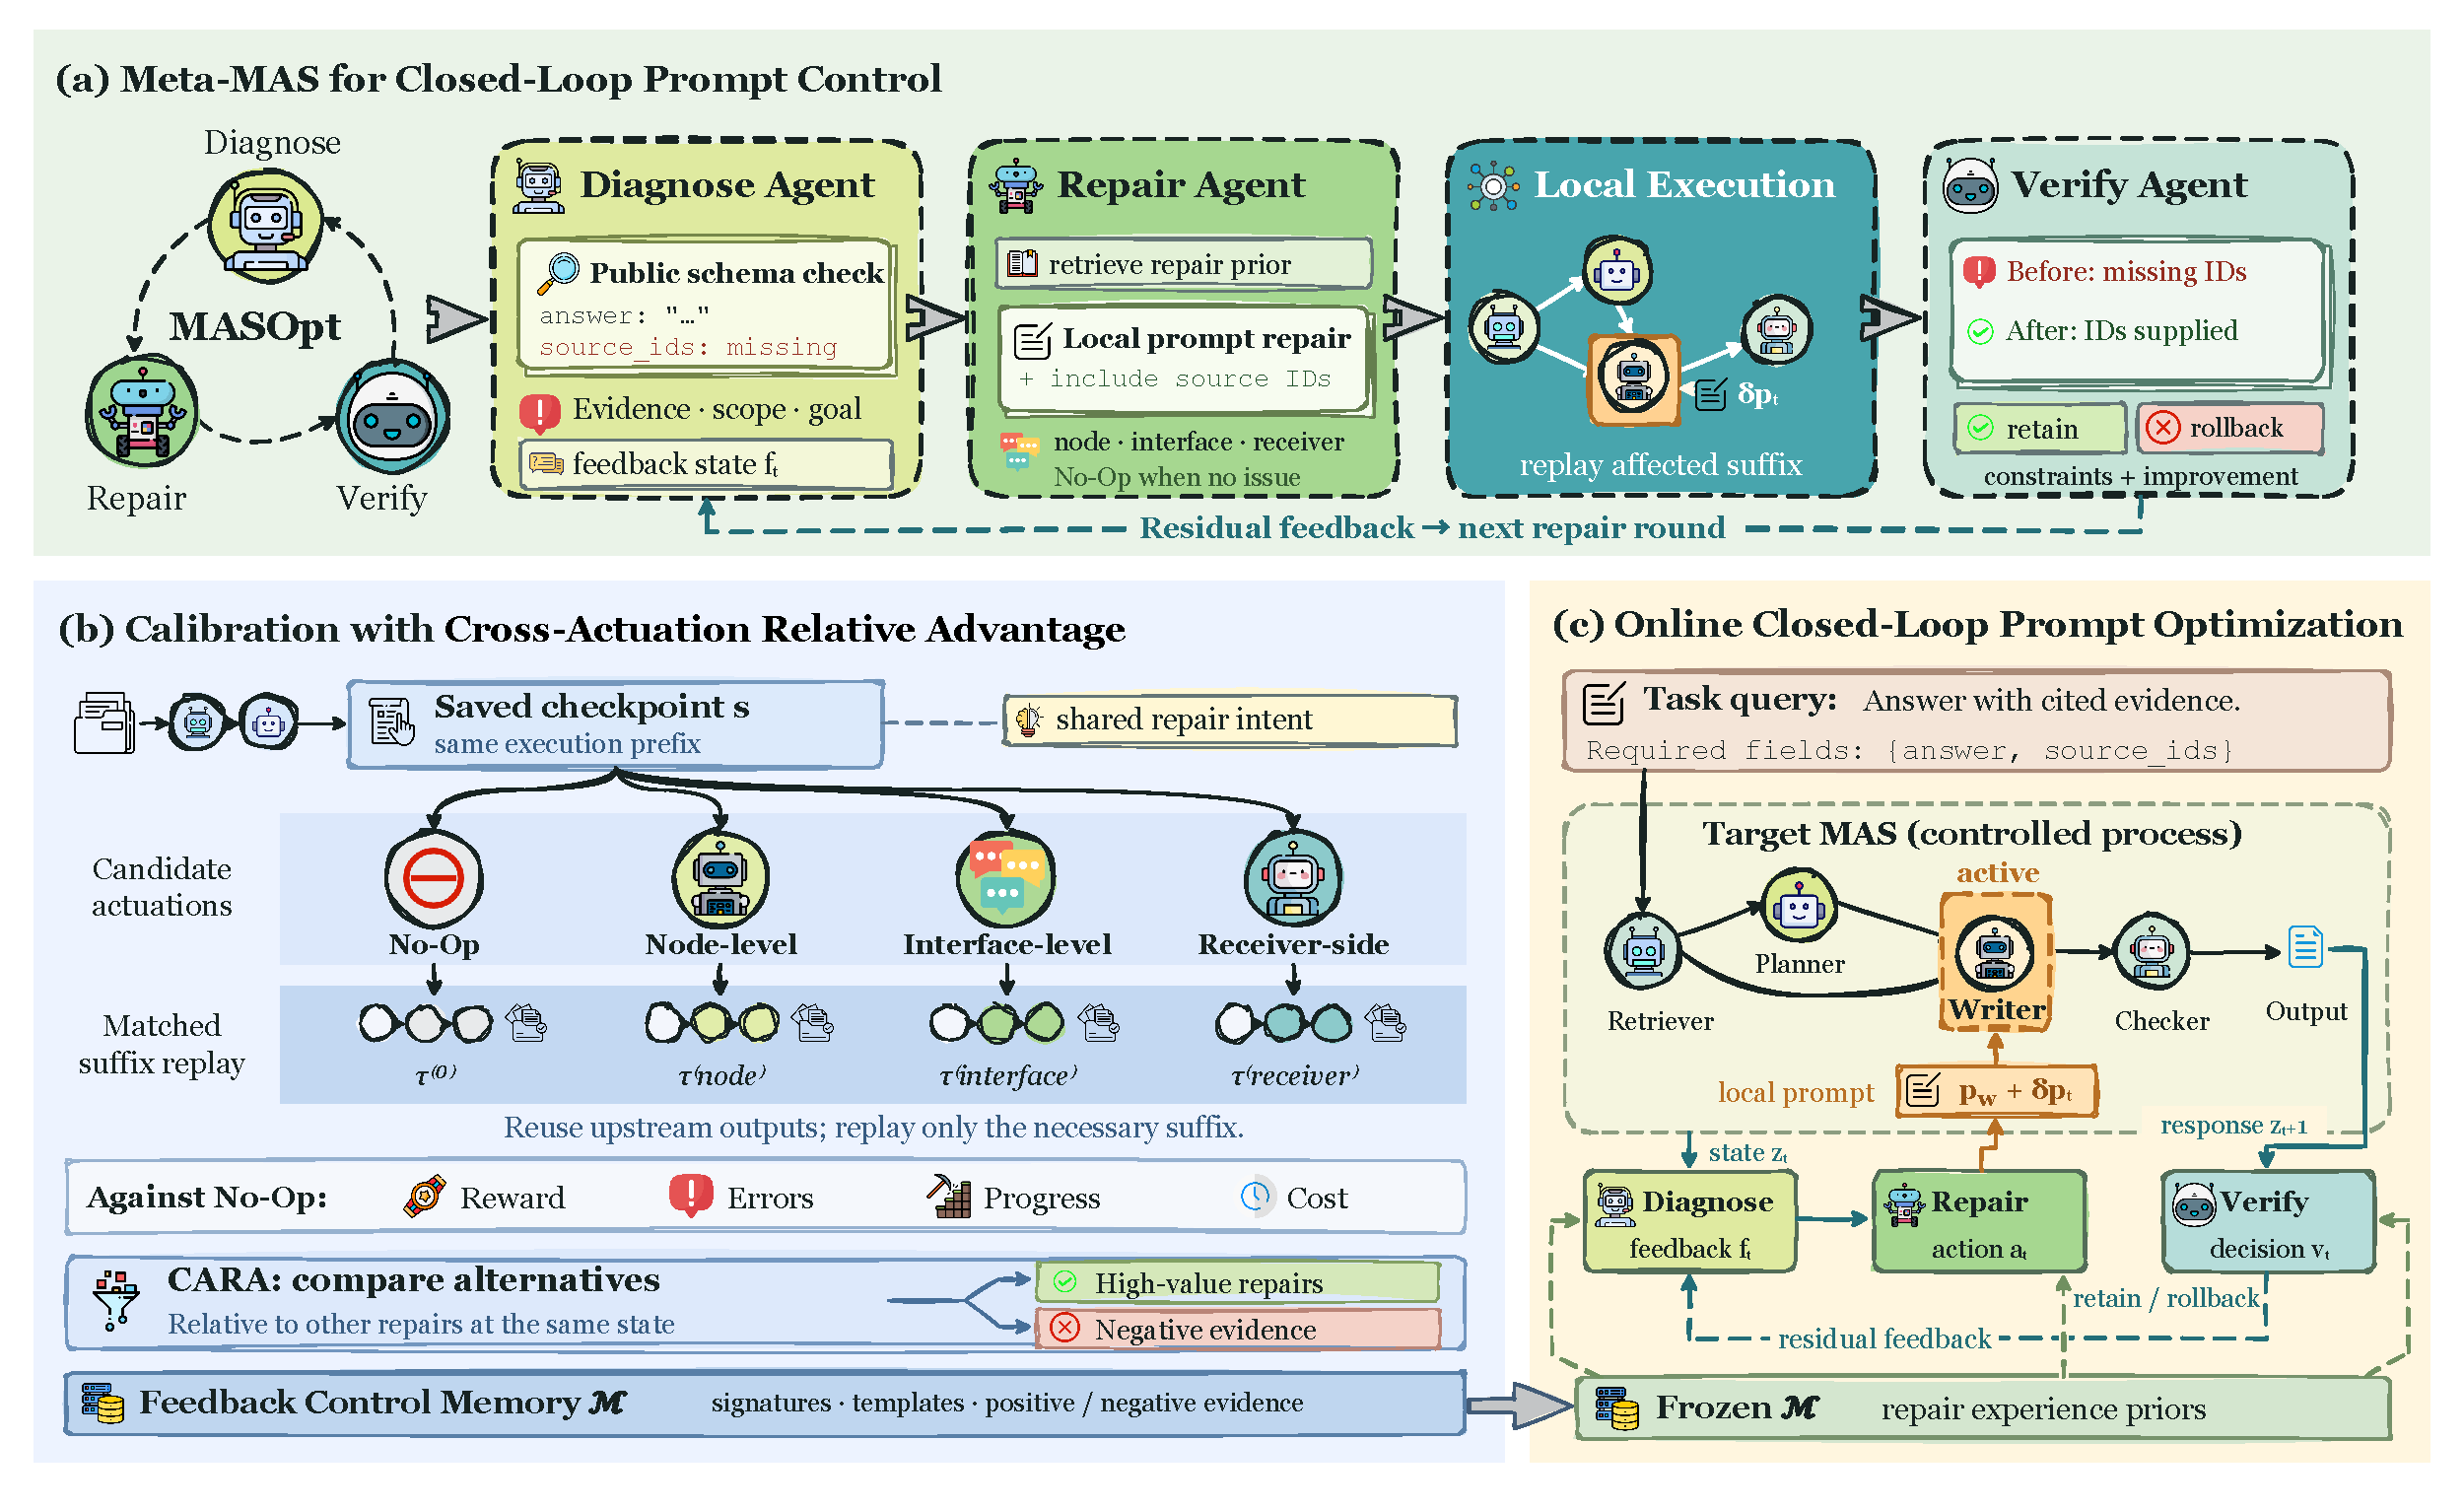
\includegraphics[width=\linewidth]{figures/masopt_method_overview.pdf}
    \caption{Overview of MASOpt. \textbf{(a) A three-agent meta-MAS for closed-loop prompt control} (Section~\ref{sec:meta_agents}): the Diagnose, Repair, and Verify Agents identify failures, propose local prompt repairs, and assess their observable effects. \textbf{(b) Offline calibration with Cross-Actuation Relative Advantage} (Section~\ref{sec:cara}): matched-state probes compare candidate actuations and distill positive and negative evidence into Feedback Control Memory. \textbf{(c) Online closed-loop prompt optimization} (Section~\ref{sec:online}): frozen memory supplies experience priors to the three agents, while prompt interventions at an active MAS node are retained or rolled back based on verification; residual feedback initiates another repair round. The task and agent roles are illustrative.}
    \label{fig:masopt-overview}
\end{figure}


\subsection{Online Prompt Optimization in Multi-Agent Systems}
\label{sec:problem}

\paragraph{Target multi-agent system.}
We consider a fixed multi-agent workflow represented by a directed graph
\begin{equation}
    \mathcal{G}=(\mathcal{V},\mathcal{E}),
\end{equation}
where each node $v_i\in\mathcal{V}$ denotes an agent invocation and each directed edge $(v_i,v_j)\in\mathcal{E}$ represents information passed from an upstream agent to a downstream agent.
The workflow topology and underlying LLMs remain fixed.
Let
\begin{equation}
    \mathbf{P}_0=
    \left(p_1^0,p_2^0,\ldots,p_N^0\right)
\end{equation}
denote the initial prompt configuration associated with the $N$ agents.

For an input task $x$, the target MAS executes according to $\mathcal{G}$ and produces a partial trajectory
\begin{equation}
    \tau_t =
    \left(o_1,o_2,\ldots,o_t\right),
\end{equation}
where $o_t$ may contain an agent response, an inter-agent message, a tool result, an environment observation, or another publicly available execution signal.
We denote the runtime information available to the optimizer by
\begin{equation}
    z_t = \mathcal{O}(x,\tau_t),
\end{equation}
where $\mathcal{O}$ excludes hidden evaluation labels and test-time ground truth.

\paragraph{Prompt intervention.}
Unlike conventional prompt optimization, MASOpt does not assume that $\mathbf{P}_0$ must remain fixed for the complete episode.
At an eligible execution checkpoint, the optimizer may apply a local prompt intervention
$a_t\in\mathcal{A}(z_t)$.
An intervention may modify the instruction of a single agent, an inter-agent interface constraint, a receiver-side rule, or a small local scope of the workflow.
A no-operation action is always available.
If an intervention is accepted, the prompt state becomes
\begin{equation}
    \mathbf{P}_{t+1}
    =
    \mathcal{U}(\mathbf{P}_t,a_t),
    \label{eq:prompt_update}
\end{equation}
where $\mathcal{U}$ applies only the local modification specified by $a_t$.

The goal is to learn an online optimization policy $\pi$ that improves final task utility while avoiding unnecessary interventions,
\begin{equation}
    \max_{\pi}\;
    \mathbb{E}_{x\sim\mathcal{D}}
    \left[
        R(\tau_T)
        -
        \lambda
        \sum_{t=1}^{T} C(a_t)
    \right],
    \qquad
    a_t\sim\pi(\cdot\mid x,z_{\leq t},\mathcal{M}),
    \label{eq:objective}
\end{equation}
where $R$ is the final task metric, $C(a_t)$ measures the cost of an intervention, and $\mathcal{M}$ denotes the repair experience obtained during offline calibration.
Importantly, $R$ is used for development-time learning and final evaluation.
The online policy does not observe hidden task labels during deployment.

\paragraph{Closed-loop view.}
Equation~\ref{eq:objective} differs from standard offline prompt search in one important respect.
The next prompt action depends on the output produced after previous actions.
From the perspective of closed-loop control theory, the target MAS acts as the controlled process, local prompt modifications serve as control inputs, and the observable trajectory provides runtime measurements.
The post-intervention response is fed back into the optimizer before another modification is made.
We use this closed-loop structure as an algorithmic principle and do not assume that LLM-based MAS satisfy linear system dynamics or classical stability conditions.


\subsection{A Three-Agent Meta-MAS for Closed-Loop Prompt Control}
\label{sec:meta_agents}

MASOpt implements the online optimizer with a lightweight meta-MAS containing three specialized agents.
They operate on the target MAS without changing its topology or model parameters.
Each agent has a narrow responsibility so that diagnosis, intervention, and verification remain separated.

\paragraph{\textbf{Diagnose Agent.}}
The Diagnose Agent converts the current execution history into a structured \emph{feedback state}.
Given the task $x$, the observable trajectory $z_{\leq t}$, and retrieved historical experience from $\mathcal{M}$, it produces
\begin{equation}
    f_t =
    \mathcal{D}
    \left(
        x,z_{\leq t};\mathcal{M}
    \right).
    \label{eq:diagnose}
\end{equation}
The feedback state records the detected problem, supporting evidence, its severity, the affected execution scope, and the behavior that should be restored.
Whenever deterministic signals are available, such as syntax errors, failed public tests, missing message fields, or invalid environment actions, they are checked before semantic diagnosis.
The Diagnose Agent therefore identifies \emph{what needs to be corrected} without committing to a particular prompt edit.

\paragraph{\textbf{Repair Agent.}}
The Repair Agent maps the feedback state to a localized prompt intervention.
It conditions on the current prompt state, the diagnosed problem, and historical repair preferences,
\begin{equation}
    a_t =
    \mathcal{R}
    \left(
        f_t,\mathbf{P}_t,z_t;\mathcal{M}
    \right).
    \label{eq:repair}
\end{equation}
Rather than rewriting the entire workflow, the Repair Agent searches over a small action space that targets only the relevant agent or communication interface.
Retrieved experience provides a prior over repair types, but the final text is instantiated using the current task context.
This design keeps interventions small and makes their effects easier to verify.

\paragraph{\textbf{Verify Agent.}}
After a candidate intervention is applied, the affected portion of the target MAS is executed again or allowed to continue until a comparable checkpoint is reached.
The Verify Agent evaluates the new observable state relative to the pre-intervention state, conditioned on applicable experience from the frozen Feedback Control Memory,
\begin{equation}
    v_t =
    \mathcal{V}
    \left(
        f_t,z_t,z_{t+1};\mathcal{M}
    \right),
    \label{eq:verify}
\end{equation}
where $v_t$ contains an acceptance decision and, when necessary, a description of the remaining problem.
Retrieved experience provides a verification prior; the acceptance decision still depends on current observable evidence and hard constraints.
A repair is retained only when the available evidence indicates improvement without violating hard constraints.
A harmful intervention is rolled back.
If the repair resolves only part of the problem, the remaining discrepancy becomes feedback for a subsequent optimization round.

The Verify Agent is therefore not merely a terminal judge.
Its post-intervention assessment determines the next state of the optimizer.
This feedback is what closes the prompt optimization loop.


\subsection{Offline Calibration with Cross-Actuation Relative Advantage}
\label{sec:cara}

Running the online optimizer without prior experience would require repeated exploration at deployment time.
MASOpt therefore uses the training split to estimate which types of local intervention are effective under different execution states.
This stage does not update any LLM parameters.
Instead, it calibrates an external feedback-control memory.

\paragraph{\textbf{Matched-state actuation probing.}}
We first execute the fixed target MAS on calibration tasks and retain a small set of informative checkpoints.
For a checkpoint $s$, MASOpt constructs a repair intent that specifies the behavior to be restored without prescribing where the repair should be applied.
It then generates a candidate set
\begin{equation}
    \mathcal{A}_s =
    \left\{
        a_0,a_1,\ldots,a_K
    \right\},
\end{equation}
where $a_0$ denotes \textsc{No-Op} and the remaining candidates correspond to legal local interventions such as node-level, interface-level, or receiver-side repairs.

All candidates are evaluated from the same saved execution prefix.
Unaffected upstream outputs are reused and only the necessary suffix is replayed.
This matched-state design controls for differences in the preceding trajectory and makes the comparison primarily reflect the effect of the intervention itself.

\paragraph{\textbf{Cross-Actuation Relative Advantage.}}
For an actuation $a$ at state $s$, we define a paired utility
\begin{equation}
\begin{split}
    U(s,a)
    =\;&
    \lambda_R \Delta R(s,a)
    +
    \lambda_E \Delta E(s,a)
    +
    \lambda_P \Delta P(s,a) \\
    &-
    \lambda_C C(s,a),
\end{split}
\label{eq:utility}
\end{equation}
where $\Delta R$ is the task-reward improvement relative to the matched \textsc{No-Op}, $\Delta E$ measures the reduction in observable execution error, $\Delta P$ measures progress toward task completion, and $C$ captures intervention and replay cost.
Ground-truth task reward is used only during offline calibration.

Absolute improvement alone is often difficult to compare across heterogeneous states.
We therefore introduce \textbf{Cross-Actuation Relative Advantage (CARA)}, which evaluates each repair relative to the other candidate interventions generated from the same checkpoint.
Let
\begin{equation}
    \mu_{-a}(s)
    =
    \frac{1}{|\mathcal{A}_s|-1}
    \sum_{\substack{b\in\mathcal{A}_s\\b\neq a}}
    U(s,b)
\end{equation}
and let $\sigma_{-a}(s)$ be the corresponding standard deviation.
CARA is defined as
\begin{equation}
    A_{\mathrm{CARA}}(s,a)
    =
    \frac{
        U(s,a)-\mu_{-a}(s)
    }{
        \sigma_{-a}(s)+\epsilon
    }.
    \label{eq:cara}
\end{equation}
CARA captures whether a repair is unusually effective for the \emph{same execution state}, rather than merely successful in absolute terms.
This distinction is useful in MAS because the component where an error becomes visible is not necessarily the location where intervention is most effective.

\paragraph{\textbf{Feedback Control Memory.}}
High-value repairs are distilled into reusable memory entries.
Each entry records a state or failure signature, the relevant topology context, a repair type, a bounded prompt template, its applicability conditions, and empirical effectiveness statistics.
Repairs that consistently degrade performance are retained as negative evidence rather than discarded.
At deployment time, this memory is frozen and queried only as a prior.
It never stores test answers and is not updated across test tasks.

The resulting memory therefore answers a compact question: given a recognizable execution problem, which form of local prompt intervention has historically been effective, and under what conditions?


\subsection{Online Closed-Loop Prompt Optimization}
\label{sec:online}

At deployment time, MASOpt starts each task from the original prompt configuration $\mathbf{P}_0$ and a frozen Feedback Control Memory $\mathcal{M}$.
No ground-truth answer or hidden evaluation result is available to the online optimizer.

The target MAS first executes normally until an eligible checkpoint is reached.
If the available deterministic and semantic evidence does not indicate a meaningful problem, MASOpt performs no intervention.
Otherwise, the Diagnose Agent constructs a feedback state and retrieves a small number of relevant repair experiences from $\mathcal{M}$.
The Repair Agent uses them to instantiate a minimal intervention for the current execution context.

The intervention is then applied only to the affected part of the workflow.
Whenever the execution environment permits checkpoint replay, unaffected upstream computations are reused.
In other settings, the system continues from the closest valid local state.
This restriction prevents an online repair from degenerating into a complete restart of the MAS.

The Verify Agent evaluates the post-repair behavior using only signals available during execution.
These may include deterministic constraints, public tests, consistency checks, tool responses, environment progress, or structured semantic feedback.
If the new state provides verified improvement, the repaired prompt state is retained.
If it degrades the observable state or violates a hard constraint, MASOpt restores the previous prompt state,
\begin{equation}
    \mathbf{P}_{t+1}
    =
    \begin{cases}
        \mathcal{U}(\mathbf{P}_t,a_t),
        & \text{if } v_t=\textsc{Accept}, \\[3pt]
        \mathbf{P}_t,
        & \text{if } v_t=\textsc{Reject}.
    \end{cases}
    \label{eq:accept}
\end{equation}
When the verification result indicates partial improvement, the remaining problem is incorporated into the next feedback state and the online optimizer may perform another bounded repair round.

This repeated use of post-intervention measurements is the defining distinction between MASOpt and one-shot prompt rewriting.
The online optimizer does not assume that its first repair is correct.
It continuously conditions future prompt decisions on the observed consequences of earlier ones.
All temporary prompt modifications are local to the current episode and are cleared when the task terminates.
As a result, MASOpt realizes online adaptation within a task while preserving a fixed target model, a fixed MAS topology, and a frozen cross-task experience memory.

\section{Experiments}
\label{sec:experiments}

We evaluate MASOpt on eight benchmarks and study the roles of diagnostic and verification experience, prompt quality, workflow architecture, and backbone model. The comparisons distinguish published baselines, selected system configurations, and exploratory follow-up analyses; detailed protocols are collected in Appendix~\ref{app:experimental-details}.

\subsection{Experimental Setup}
\label{sec:experimental-setup}

\paragraph{Benchmarks.}
We evaluate MASOpt on eight benchmarks spanning four domains: code generation (HumanEval and MBPP), mathematical reasoning (GSM8K and MATH Level-5), reading comprehension (HotpotQA and DROP), and interactive task completion (ALFWorld and TextCraft) \citep{chen2021humaneval,austin2021mbpp,cobbe2021gsm8k,hendrycks2021math,yang2018hotpotqa,dua2019drop,shridhar2020alfworld,prasad2024textcraft}. This suite tests both final-answer quality and adaptation to evolving environment feedback. Dataset sizes, splits, and the MATH subset composition are provided in Appendix~\ref{app:data-splits}.

\paragraph{Baselines.}
We compare three groups of methods: direct and reasoning-based prompting (IO, CoT, and ReAct), prompt optimization (PromptBreeder, Instinct, MIPRO, and MASPOB), and workflow generation or adaptation (AFlow and HiveMind). References are given alongside the methods in Table~\ref{tab:main-results}. The eight IO--MASPOB results are published means reported by \citet{hong2026maspob}; HiveMind is our unofficial three-node transfer from its original financial-trading setting. Within-system analyses compare MASOpt with the same locally executed workflow. Protocol and selection differences are documented in Appendix~\ref{app:protocols}.

\paragraph{Metrics.}
We report pass@1 on HumanEval and MBPP, answer accuracy on GSM8K and MATH, normalized F1 on HotpotQA and DROP, and native task success rate on ALFWorld and TextCraft. Internal generation branches and repair attempts do not count as additional submissions for pass@1. Task scores use a 0--100 scale, and differences are expressed in percentage points (pp); each table average weights its benchmark columns equally. Prompt quality is assessed separately with a 0--10 rubric and anonymous paired evaluation in both presentation orders.

\paragraph{Implementation details.}
Unless otherwise stated, local main, component, and architecture experiments request \texttt{gpt-4o-mini-2024-07-18} with temperature 0 and top-$p$ 1; the provider generally returns the \texttt{gpt-4o-mini} alias, so the served snapshot is not independently verified. Backbone parameters remain fixed, and hidden answers are excluded from online acceptance decisions. ALFWorld and TextCraft use 35- and 20-step limits, respectively, with at most two repair proposals in the controlled TextCraft runs. Local scores normally summarize one complete prediction set, and the main MASOpt row selects the highest completed score per task. Because some development used test-set feedback, these results characterize the recorded systems rather than an untouched holdout; split allocations, model-selection history, and budget differences are detailed in Appendix~\ref{app:protocols}.

\subsection{Main Results}
\label{sec:main-results}

\begin{table}[!htbp]
    \centering
    \setlength{\belowcaptionskip}{6pt}
    \caption{Performance (\%) on six non-interactive benchmarks. Baselines are ordered by increasing reported average; MASOpt is separated and bolded. All baselines except HiveMind use published means from \citet{hong2026maspob}, with dispersion omitted; HiveMind is a local adaptation. MASOpt reports selected completed configurations. Avg. is the unweighted six-benchmark mean. See Appendix~\ref{app:protocols} for comparability limits.}
    \label{tab:main-results}
    \scriptsize
    \setlength{\tabcolsep}{3.7pt}
    \resizebox{\textwidth}{!}{%
    \begin{tabular}{@{}lccccccc@{}}
        \toprule
        Method & HumanEval & MBPP & GSM8K & MATH & HotpotQA & DROP & Avg. \\
        \midrule
        IO (GPT-4o-mini) & 89.31 & 69.11 & 87.80 & 51.71 & 60.36 & 53.09 & 68.56 \\
        CoT \citep{wei2022cot} & 89.57 & 69.89 & 88.34 & 52.47 & 67.62 & 58.27 & 71.03 \\
        ReAct \citep{yao2023react} & 87.79 & 66.08 & 88.91 & 52.61 & 65.61 & 67.25 & 71.38 \\
        PromptBreeder \citep{fernando2024promptbreeder} & 88.80 & 70.38 & 91.97 & 52.13 & 68.76 & 71.85 & 73.98 \\
        Instinct \citep{lin2023instinct} & 90.08 & 70.23 & 92.64 & 52.40 & 69.92 & 71.90 & 74.53 \\
        AFlow \citep{zhang2024aflow} & 91.09 & 79.96 & 93.36 & 53.83 & 73.42 & 79.48 & 78.52 \\
        MIPRO \citep{opsahlong2024mipro} & 91.35 & 80.65 & 92.80 & 54.90 & 74.37 & 79.13 & 78.87 \\
        HiveMind \citep{xia2025hivemind} & 89.31 & 71.55 & 92.99 & 57.41 & 67.23 & 68.76 & 74.54 \\
        MASPOB \citep{hong2026maspob} & 94.15 & 80.65 & 93.90 & 57.05 & 75.43 & 82.28 & 80.58 \\
        \midrule
        \textbf{MASOpt} & \textbf{96.95} & \textbf{84.16} & \textbf{94.41} & \textbf{62.76} & \textbf{76.49} & \textbf{85.66} & \textbf{83.40} \\
        \bottomrule
    \end{tabular}}
\end{table}

\paragraph{Observation 1: Broad performance gains across non-interactive tasks.}
Table~\ref{tab:main-results} shows that the selected MASOpt configurations attain the highest reported score on all six benchmarks, with an average of 83.40 versus 80.58 for MASPOB. Relative to MASPOB, the gains are 2.80/3.51 pp on HumanEval/MBPP, 0.51/5.71 pp on GSM8K/MATH, and 1.06/3.38 pp on HotpotQA/DROP. The larger gains on MATH and MBPP contrast with the smaller margin on GSM8K, where the baseline already reaches 93.90. This pattern is consistent with task-dependent opportunities for local repair. These are descriptive comparisons of selected MASOpt configurations with published baseline means, not a matched statistical test.

\begin{wraptable}{r}{0.50\textwidth}
    \vspace{-\intextsep}
    \centering
    \caption{Interactive success rate (\%). Avg. weights the three score columns equally. ALFWorld uses historical archives; TextCraft uses the shared action interface. Protocol differences are detailed in Appendix~\ref{app:interactive-protocols}.}
    \label{tab:interactive-results}
    \small
    \setlength{\tabcolsep}{2.3pt}
    \renewcommand{\arraystretch}{1.04}
    \begin{tabular*}{\linewidth}{@{\extracolsep{\fill}}lrrrr@{}}
        \toprule
        & \multicolumn{2}{c}{ALFWorld} & & \\
        \cmidrule(lr){2-3}
        Method & Seen & Unseen & TextCraft & Avg. \\
        \midrule
        HiveMind & 28.57 & 27.61 & 12.50 & 22.89 \\
        MASPOB & 47.86 & 50.75 & 13.75 & 37.45 \\
        MIPRO & 51.43 & 50.00 & 12.50 & 37.98 \\
        AFlow & 50.71 & 54.48 & 12.50 & 39.23 \\
        \midrule
        \textbf{MASOpt} & \textbf{75.00} & \textbf{89.55} & \textbf{30.00} & \textbf{64.85} \\
        \bottomrule
    \end{tabular*}
    \vspace{-0.5\baselineskip}
\end{wraptable}

\paragraph{Observation 2: Higher recorded success on interactive tasks.}
Table~\ref{tab:interactive-results} extends the comparison to sequential decisions. MASOpt solves 24 of 80 TextCraft tasks (30.00\%), compared with 10 for MIPRO and 11 for the simplified MASPOB adaptation, under the shared typed action interface and 20-step limit. Its historical ALFWorld scores are 75.00\% on seen tasks and 89.55\% on unseen tasks, giving a three-column average of 64.85. These observations motivate local repair from dependency, inventory, and environment feedback. However, the ALFWorld baseline names identify seed-plus-memory archives with identical role prompts, not distinct optimizer executions; a later MASOpt rerun reaches 84.33\% on unseen tasks. Appendix~\ref{app:interactive-protocols} reports these distinctions and the associated interaction costs, so the historical margins should not be read as controlled algorithmic gains.

\FloatBarrier
\subsection{Contribution of Diagnostic and Verification Experience}
\label{sec:experience-ablation}

We examine whether learned experience helps the controller locate failures and decide which repairs to retain. This study separates the contribution of diagnostic and verification experience from the effect of simply invoking the three-agent control loop.

\begin{figure}[!htbp]
    \centering
    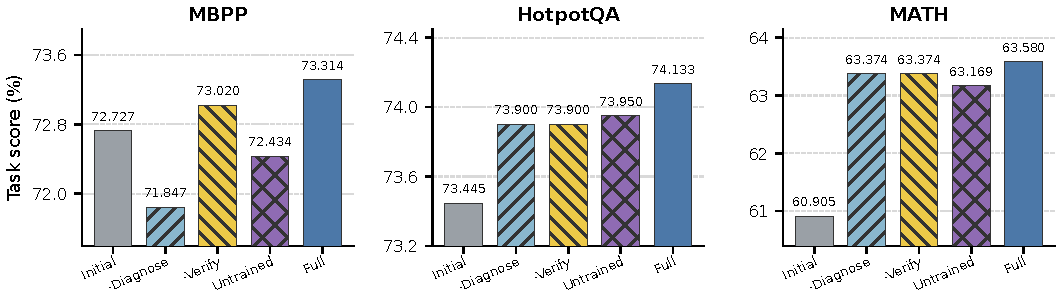
\includegraphics[width=0.94\textwidth]{figures/ablation_experience.pdf}
    \caption{Experience ablations on MBPP (341 tasks), HotpotQA (800), and MATH (486). Each panel uses a dataset-specific truncated vertical axis to make sub-point differences visible; bar labels are rounded to three decimals. GSM8K is omitted because its separately registered controller is not structurally identical to these three runs.}
    \label{fig:experience-ablation}
\end{figure}

We compare Full with variants that remove diagnostic experience, verification experience, or all learned experience while retaining the controller and its underlying workflow. All variants share the same configuration-specific Initial outputs. As shown in Figure~\ref{fig:experience-ablation}, Full improves over Initial by 0.59, 0.69, and 2.67 pp on MBPP, HotpotQA, and MATH, and exceeds the strongest displayed ablation by 0.29, 0.18, and 0.21 pp. Removing diagnostic experience produces the largest MBPP decrease (1.47 pp); on MATH, removing either diagnostic or verification experience changes only one correct answer. Thus, the recorded benefit varies by task and is modest in several comparisons. These post-hoc results are exploratory; configuration-specific baselines, fallback behavior, and the separate GSM8K analysis are documented in Appendix~\ref{app:experience-details}.

\begin{figure}[!htbp]
    \centering
    \begin{minipage}[t]{0.49\textwidth}
        \vspace{0pt}
        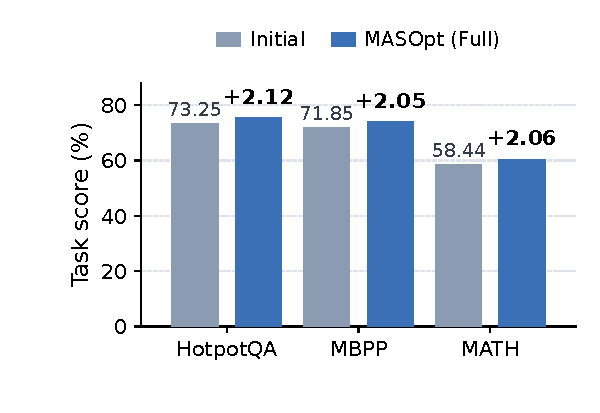
\includegraphics[width=\linewidth]{figures/architecture_adaptation.pdf}
        \caption{Adaptation to three alternative workflows. Gray bars show Initial and blue bars Full; labels give Initial scores and Full-minus-Initial gains in pp.}
        \label{fig:architecture-adaptation}
    \end{minipage}\hfill
    \begin{minipage}[t]{0.49\textwidth}
        \vspace{0pt}
        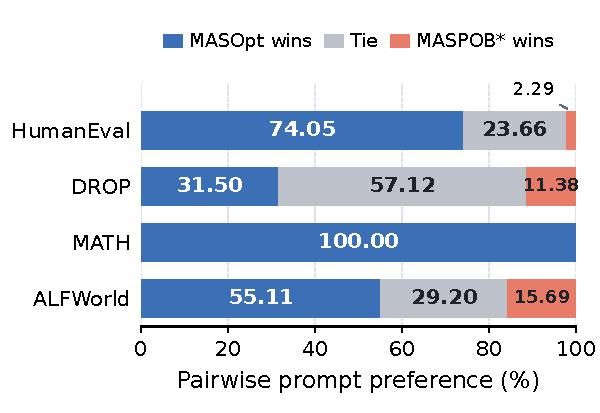
\includegraphics[width=\linewidth]{figures/prompt_quality.pdf}
        \caption{Pairwise prompt preference on four datasets. Segments show MASOpt wins, ties, and MASPOB* wins; zero-width segments are omitted.}
        \label{fig:prompt-quality}
    \end{minipage}
\end{figure}

\subsection{Pairwise Prompt Quality}
\label{sec:prompt-quality}

We examine whether MASOpt prompts are preferred under a fixed rubric independently of final task success. This study compares paired prompts on HumanEval, DROP, MATH, and ALFWorld to assess instruction quality across code generation, reading comprehension, mathematical reasoning, and interactive decision-making.

A GPT-5.6-sol judge scores anonymized prompts in both A/B and B/A orders on six 0--10 dimensions. We average the two overall-quality scores for each prompt; a MASOpt-minus-baseline difference above 0.5 is a win, below $-0.5$ is a loss, and otherwise is a tie. MASPOB* uses the published optimized prompts on the three non-interactive datasets and a seed-plus-memory archive on ALFWorld. Figure~\ref{fig:prompt-quality} shows MASOpt win rates of 74.05\%, 31.50\%, 100.00\%, and 55.11\%, respectively. MATH receives uniform preference, while DROP is dominated by ties (57.12\%), indicating a weaker separation under the rubric. On ALFWorld, MASOpt wins exceed baseline wins (15.69\%), with 29.20\% ties. These selected-dataset comparisons provide evidence about judged prompt quality, not task success; a single evaluator and presentation-order sensitivity limit the strength of the conclusion.

\subsection{Adaptation to Alternative Workflow Architectures}
\label{sec:architecture-adaptation}

We test whether MASOpt remains useful when the underlying workflow is simplified. By holding the backbone and task set fixed while changing the branch structure, this study examines the controller's applicability beyond the original workflow configuration.

We use one \textsc{AnswerGenerate} call followed by \textsc{FormatAnswer} on HotpotQA, one \textsc{CodeGenerate} branch followed by test and repair on MBPP, and two text solvers with \textsc{ScEnsemble} but no program branch on MATH. Initial executes each alternative workflow directly; Full applies MASOpt to the same workflow. Figure~\ref{fig:architecture-adaptation} compares the fixed Initial scores with the latest Full results: 73.2481 to 75.3711 on HotpotQA, 71.8475 to 73.9003 on MBPP, and 58.4362 to 60.4938 on MATH. The corresponding gains are 2.12, 2.05, and 2.06 pp. The similar positive margins suggest that local repair remains useful across these three branch structures. The recorded configurations include post-hoc policy choices and execution recovery, so the comparison supports applicability to the tested workflows rather than architecture-independent improvement under a uniform budget.

\FloatBarrier
\subsection{Adaptation Across Backbone Models}
\label{sec:backbone-adaptation}

We examine whether MASOpt can be instantiated with different backbone models while retaining the same online repair mechanism. This study characterizes model-specific adaptation across six benchmarks, rather than assuming that a controller calibrated for one backbone transfers unchanged.

\begin{figure}[!htbp]
    \centering
    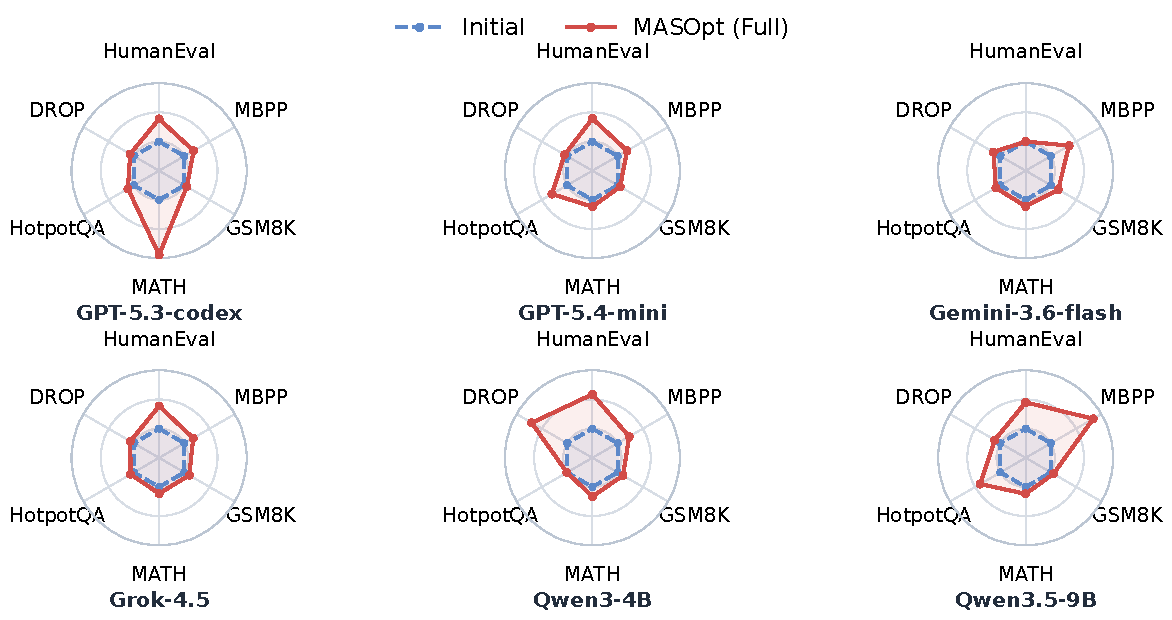
\includegraphics[width=\textwidth]{figures/backbone_radar.pdf}
    \caption{Adaptation across six backbones. Each Initial score is normalized to 100; all panels use the same 99--102 radial range to resolve small differences.}
    \label{fig:backbone-radar}
\end{figure}

We pair each model-specific Initial workflow with its Full counterpart on HumanEval, MBPP, GSM8K, MATH, HotpotQA, and DROP. Figure~\ref{fig:backbone-radar} compares the six backbones under these paired configurations. Full improves in 35 of 36 model--task pairs and ties Gemini-3.6-flash on HumanEval, where Initial already reaches 100\%. Mean gains across the six tasks range from 0.25 to 0.51 pp across backbones. The pattern shows broadly positive but modest and task-dependent changes. Experience, recovery policies, and execution budgets differ across configurations, so these results support model-specific applicability rather than controlled transfer or statistically significant improvement under a common protocol. Appendix~\ref{app:backbone-protocols} details these differences.

\FloatBarrier

\section{Conclusion}
\label{sec:conclusion}

We presented MASOpt, a framework for online prompt optimization in multi-agent systems. MASOpt treats prompt edits as local control actions, separates diagnosis, repair, and verification, and uses Cross-Actuation Relative Advantage to transfer repair preferences from matched execution states. This formulation preserves the target models and workflow topology while allowing the prompt state to adapt within an episode.

The empirical section is intentionally left open until the planned benchmark runs are complete. Once those experiments are available, the analysis should focus on when online repair is useful, how much intervention cost it incurs, and whether CARA improves the efficiency and reliability of closed-loop optimization. These questions are central to determining the practical scope of MASOpt.


\subsection*{AI use statement}

Generative AI tools were used for language editing and LaTeX organization during manuscript preparation. The authors reviewed all AI-assisted text, verified the cited sources, and take responsibility for the final manuscript and its claims.

\subsection*{Ethics statement}

This work uses publicly available benchmarks and does not involve human subjects, private data, or interventions in real-world decision-making. The authors will document model access, evaluation procedures, and failure cases to support responsible use of online prompt adaptation.

\subsection*{Reproducibility statement}

The method is specified in Sections~\ref{sec:method} and the planned evaluation protocol is described in Section~\ref{sec:experiments}. The final version will release the prompt templates, calibration trajectories, evaluation scripts, and configuration files needed to reproduce the reported results, subject to the terms of the underlying model and benchmark licenses.

\bibliography{iclr2027_conference}
\bibliographystyle{iclr2027_conference}

\appendix
% Additional experimental details will be included with the final benchmark results.


\section{Experimental Details}
\label{app:experimental-details}

\subsection{Datasets and Splits}
\label{app:data-splits}

Table~\ref{tab:data-splits} lists the data pools and evaluation metrics. Following AFlow, the fixed MATH Level-5 test subset contains 155 Prealgebra, 124 Number Theory, 108 Precalculus, and 99 Counting \& Probability problems. Development-pool sizes describe the available data, rather than a shared optimization protocol for all historical configurations.

\begin{table}[!htbp]
    \centering
    \setlength{\belowcaptionskip}{6pt}
    \caption{Datasets, local splits, and evaluation metrics. HumanEval uses five registered development-fold configurations over 33 problems and a fixed 131-problem test set. All reported scores are on a 0--100 scale.}
    \label{tab:data-splits}
    \footnotesize
    \setlength{\tabcolsep}{7pt}
    \resizebox{\textwidth}{!}{%
    \begin{tabular}{@{}llrrl@{}}
        \toprule
        Task family & Benchmark & Development pool & Test size & Metric \\
        \midrule
        Code generation & HumanEval & 33 & 131 & pass@1 \\
                        & MBPP & 86 & 341 & pass@1 \\
        Mathematical reasoning & GSM8K & 264 & 1,055 & answer accuracy \\
                               & MATH & 119 & 486 & answer accuracy \\
        Reading comprehension & HotpotQA & 200 & 800 & token F1 \\
                              & DROP & 200 & 800 & answer F1 \\
        Interactive environments & ALFWorld & 33 training tasks & 140 seen / 134 unseen & task success rate \\
                                 & TextCraft & 20 & 80 & task success rate \\
        \bottomrule
    \end{tabular}}
\end{table}

\subsection{Implementation and Selection Protocols}
\label{app:protocols}

Table~\ref{tab:main-results} reproduces the means of eight literature baselines from \citet{hong2026maspob}; their reported standard deviations are omitted. The \emph{Original workflow} in within-system comparisons is the locally executed graph with its original role prompts. Our HiveMind result is an unofficial three-node transfer of a method originally developed for a seven-agent financial trading system: two independent analysis nodes feed an integrator, and exact DAG-Shapley contribution, cached identical inputs, lowest-contribution selection, and success/failure reflection are retained while task score replaces the original coalition reward. This local transfer uses a fixed 20-example development subset in four five-example update windows, whereas the selected historical MASOpt systems have a different model-selection history. We therefore do not present this implementation as an official reproduction or an equal-budget comparison.

Unless stated otherwise, local main, component, and architecture experiments requested \texttt{gpt-4o-mini-2024-07-18} with temperature 0 and top-$p$ 1. The provider generally returned the \texttt{gpt-4o-mini} alias, so the underlying served snapshot was not independently verified. MASOpt never updates backbone parameters. Reference answers and benchmark scores are used for offline reward construction and evaluation, but are not exposed to the online acceptance rule.

For experience construction, selection, and controller selection, respectively, the local development pools are split 140/30/30 for HotpotQA and DROP, 184/39/41 for GSM8K, 83/17/19 for MATH, and 60/12/14 for MBPP; HumanEval uses five registered folds. The imported MBPP workflow also uses additional public checks and experience drawn from the 86-problem development pool, so its comparison with the original workflow is not a controlled contrast in which both systems see only examples attached to the test problem. ALFWorld runs use a 35-step limit. The controlled TextCraft runs use 20 environment steps and at most two repair proposals. Each non-interactive HiveMind test item uses three node calls with at most 4,096 output tokens per call; interactive calls use at most 1,024 output tokens per node and the corresponding 35/20-step limits. Unless otherwise noted, each local score is computed from one complete set of task predictions rather than repeated random-seed runs.

Some historical development and follow-up analyses used feedback from the same test set that is reported below. Regenerating predictions does not restore that set as an untouched holdout. We therefore use these experiments to characterize the implemented systems and mechanisms, not to claim unbiased estimates of generalization after model selection.

\subsection{Interactive Evaluation Protocols}
\label{app:interactive-protocols}

On TextCraft, MIPRO, the simplified MASPOB adaptation, and MASOpt solve 10, 11, and 24 of 80 tasks, respectively. All three use the same recipe-ID/material-binding interface and native environment success condition. MIPRO performs ten trials of categorical TPE search over instructions and examples; MASPOB performs 36 UCB prompt-arm trials without its GNN; MASOpt adds targeted repair from public dependency and inventory constraints. The frozen MASOpt controller can still generate task-local repairs from public observations, but it does not update cross-task memory or select prompts using test accuracy. The complete tests use 699, 684, and 888 API calls, respectively. Across development, search, initial, and repaired runs, the archived TextCraft campaign records 4,923 physical calls and 13,114,187 known tokens; token counts for three retried network failures are unavailable.

The ALFWorld labels for AFlow, MIPRO, and MASPOB denote seed-plus-static-memory archives whose four role prompts are identical, rather than executions of three distinct optimizers; their score differences must not be attributed to the named algorithms. The latest verified MASOpt rerun obtains 105/140 (75.00\%) on seen tasks and 113/134 (84.33\%) on unseen tasks, whereas Table~\ref{tab:interactive-results} retains the historical 75.00/89.55 configuration. All 274 rerun receipts agree with the native terminal \texttt{won} field, although action guards override 43.88\% and 50.46\% of seen and unseen actions. For context, A$^2$Flow \citep{zhao2025a2flow}, using DeepSeek-v3 and a different protocol, reports 25.0\%, 31.3\%, and 59.0\% on ALFWorld seen, ALFWorld unseen, and TextCraft. The model, interface, and interaction budgets differ, so this is not a like-for-like comparison.

\subsection{Experience Ablation: Configuration Details}
\label{app:experience-details}

We compare the full controller with three ablations: removing experience from the Diagnose Agent, removing experience from the Verify Agent, and removing all learned experience and the experience-memory component from the three-agent controller. The last variant still invokes Diagnose, RepairExecute, and Verify and then calls the underlying task workflow; it is therefore not a three-call replacement for the complete system. Within each registered dataset configuration, all arms reuse the same Initial outputs. These are post-hoc exploratory runs and do not replace the main configurations in Table~\ref{tab:main-results}.



Figure~\ref{fig:experience-ablation} shows that Full improves over its paired Initial by 0.5865 pp on MBPP, 0.6880 pp on HotpotQA, and 2.6749 pp on MATH. Among the displayed ablations, Full is higher than the strongest ablated arm by 0.2933, 0.1835, and 0.2058 pp, respectively. On MBPP, removing diagnostic experience causes the largest decrease relative to Full (1.4663 pp). On MATH, removing either diagnostic or verification experience changes one correct answer relative to Full. These effects are heterogeneous and small in several cells; they do not by themselves identify a stable causal contribution. The MBPP verification ablation also contains fallback behavior after selector-parsing failures, while the latest MATH controller includes deterministic arithmetic-candidate generation.

The paired Initial is configuration-specific and is not always the untouched original prompt. In particular, HotpotQA uses the original \texttt{round\_1} output (73.4451), whereas an independently regenerated original baseline scores 73.9734 but has no matched Full run. MATH uses a \texttt{round\_1} graph with a finalization wrapper and scores 60.9053; an independent original-prompt baseline scores 62.3457 but likewise cannot replace the paired Initial. On the separately registered GSM8K controller, Initial and Full score 93.2701 and 93.6493: Full repairs seven examples and harms three, but its score equals the best ablation. A prior verifier version scored 92.6066 after repairing seven and harming fourteen examples. This history further motivates treating the study as exploratory.

\subsection{Backbone Adaptation: Evidence and Protocol Differences}
\label{app:backbone-protocols}

Finally, we evaluate GPT-5.3-codex, GPT-5.4-mini, Gemini-3.6-flash, Grok-4.5, Qwen3-4B, and Qwen3.5-9B on all six non-interactive benchmarks. Each model uses its own recorded experience, prompts, output budget, recovery path, and terminal policy. The study therefore measures adaptation of complete model-specific systems rather than a single-factor backbone substitution.

These evaluations also involve departures from a uniform protocol. Qwen3.5-9B on MATH uses host-side symbolic computation, and the source Grok-4.5 MATH recovery run uses four calls rather than the registered two-call budget. The added 18 cells on MBPP, GSM8K, and HotpotQA reuse valid historical predictions where available, recover missing outputs, and, for configurations that had not improved, apply terminal prompts or acceptance rules informed by observed errors. Those cells are post-hoc analyses on the original test denominators, not confirmatory results on an untouched test set. The uniformly non-negative pattern therefore documents the scope of the current model-specific implementations; it does not prove transfer under a common budget or isolate the causal effect of changing only the backbone.



\end{document}
